\chapter{Firewalls, IDS and Web Security}
\section{Firewalls}
Un firewall è un componente passivo di difesa perimetrale di una rete informatica, che integra un insieme di misure progettate per prevenire l'accesso non autorizzato a tale rete. Letteralmente firewall significa \textit{muro tagliafuoco}, con riferimento ai muri refrattari costruiti nelle strutture per assicurarne l'isolamento.

\subsection{Firewall Policies}
Al fine di proteggere reti private o singole macchine dai pericoli di Internet, un firewall può essere utilizzato per filtrare il traffico in uscita o in entrata sulla base di un insieme di regole predefinite, denominate \textbf{firewall policies}.
I pacchetti che passano per un firewall possono essere:
\begin{itemize}
\item \textbf{Accepted}: il firewall ne permette il passaggio
\item \textbf{Dropped}: il passaggio non viene permesso e tale negazione non viene segnalata
\item  \textbf{Rejected}: il passaggio non viene permesso e il firewall tenta di informare la sorgente del pacchetto del rifiuto
\end{itemize}
Le policies usate dal firewall per gestire il traffico sono basate su diverse proprietà dei pacchetti che vengono analizzati, incluso il protocollo usato, come:
\begin{itemize}
\item TCP o UDP
\item Gli indirizzi IP del mittente e del destinatario
\item Le porte di partenza e di destinazione del pacchetto
\item il payload del livello applicativo del pacchetto (ad esempio analizzando se contiene virus)
\end{itemize}
\subsubsection{Blacklist e Whitelist}
Vi sono due approcci fondamentali nella creazione delle policies che garantiscono la minimizzazione delle vulnerabilità esposte pur mantenendo le funzionalità desiderate:

\begin{itemize}
\item \textbf{Blacklist approach}: Tutti i pacchetti sono accettati, tranne quelli per cui sono verificate le condizioni specificate nella blacklist. Questo tipo di configurazione, \textbf{orientata al servizio}, è più flessibile nell'assicurare che le funzionalità desiderate non siano danneggiate dal firewall, ma dal punto di vista di vista della sicurezza risulta un approccio "ingenuo": si assume che l'amministratore conosca tutte le proprietà a cui può rispondere l'eventuale traffico malevolo.

\item \textbf{Whitelist approach}: Un approccio più sicuro, \textbf{orientato alla sicurezza}, consiste nel rifiutare il traffico per default, in modo che i pacchetti siano rifiutati a meno che non rispondano a determinate condizioni specificate dal firewall. 
\end{itemize}

\subsection{Tipi di Firewall}
\begin{itemize}
\item \textbf{packet filters (stateless)}: Se un pacchetto soddisfa le regole definite dal packet filter, viene trattato di conseguenza (rifiutato o accettato a seconda dell'approccio utilizzato, i.e. blacklist o whitelist)
\item \textbf{"stateful" filters}: Questo tipo di firewall tiene traccia di tutte le connessioni che passano attraverso di esso, e può determinare se un pacchetto corrisponde all'apertura di una nuova connessione, se appartiene ad una connessione precedente o se è un pacchetto invalido.
\item \textbf{application layer}: Questo tipo di firewall funziona come un proxy, in modo da poter "capire" determinati protocolli o applicazioni. Può analizzare il contenuto del traffico, eventualmente bloccandolo in caso di contenuti sospetti (i.e. siti web, virus, vulnerabilities, ...).
\end{itemize}
\subsubsection{Stateless firewalls (Packet filters)}
Un firewall stateless non tiene in memoria nessuno stato rispetto ai pacchetti che processa. Tratta ogni pacchetto indipendentemente ed in maniera isolata dagli altri, senza considerare, ad esempio, se ha già processato lo stesso pacchetto in passato. \textbf{In genere i firewall stateless devono essere configurati in maniera abbastanza restrittiva affinché prevengano la maggior parte degli attacchi.}

\begin{figure}[htbp]
	\centering%
	\subfigure%
	{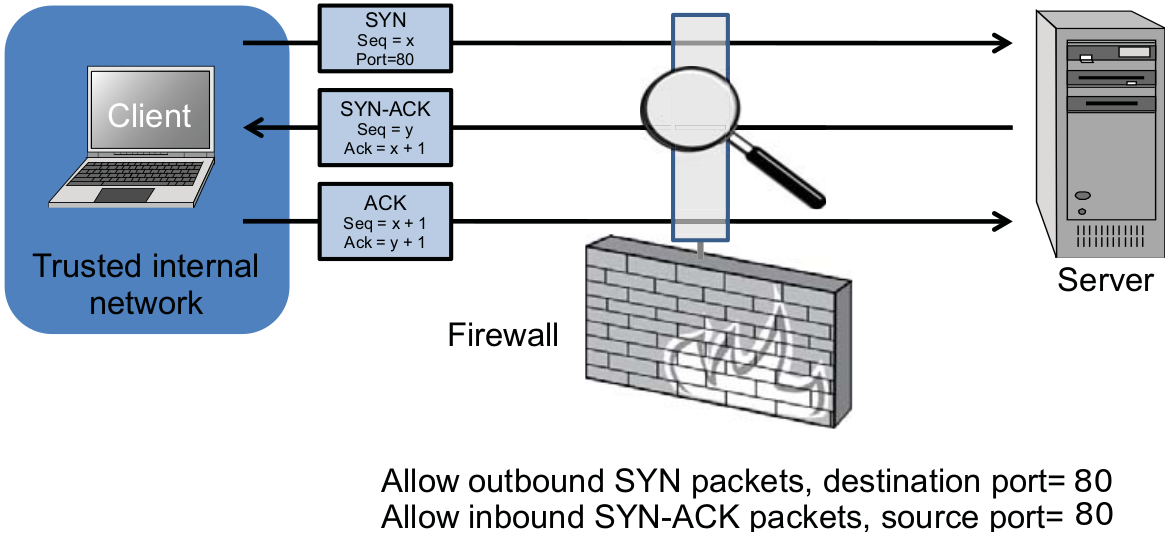
\includegraphics[height=13cm, width=13cm, keepaspectratio]{Immagini/firewalls/stateless_firewall.png}}
	\caption{Stateless firewall \label{fig:stateless_firewall}} 	
\end{figure}

\subsubsection{Stateful firewalls}
I firewall stateful sono in grado di riconoscere i pacchetti che fanno parte di una sessione legittima originata all'interno di una rete fidata. Essi tengono in memoria tabelle contenenti informazioni su ogni connessione attiva, come indirizzi IP, porte e numeri di sequenza dei pacchetti. Usando tali tabelle, questo tipo di firewall può permettere, ad esempio, solo il passaggio di pacchetti che rappresentano una risposta ad una connessione iniziata dall'interno della rete fidata.

\begin{figure}[htbp]
	\centering%
	\subfigure%
	{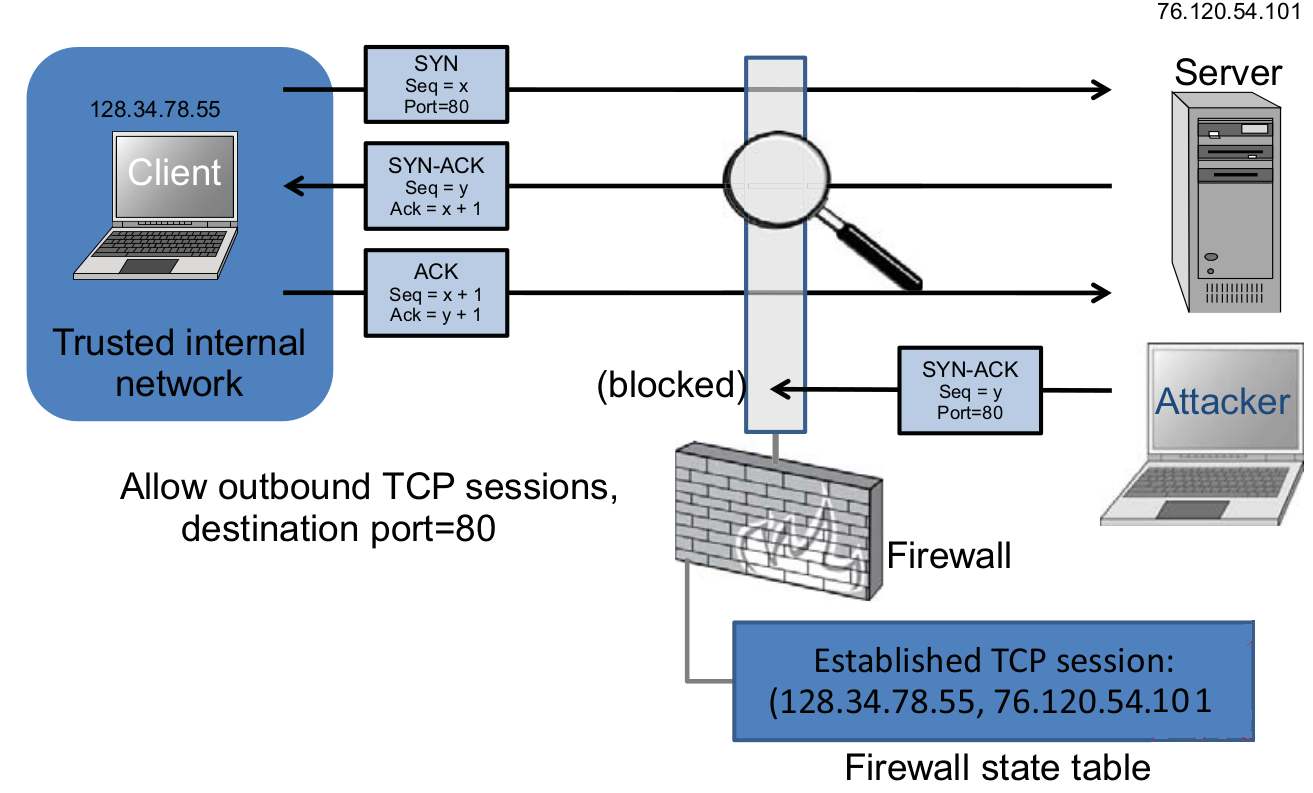
\includegraphics[height=13cm, width=13cm, keepaspectratio]{Immagini/firewalls/stateful_firewall.png}}
	\caption{Stateful firewall \label{fig:stateful_firewall}} 	
\end{figure}

\section{Tunnels}
Il contenuto dei normali pacchetti TCP non è solitamente crittografato. Se qualcuno pratica eavesdropping sulla connessione può spesso vedere il completo contenuto dei payloads della sessione. Un modo per prevenire questo tipo di attacco alla confidenzialità senza modifificare lo strato applicativo coinvolto nella sessione è utilizzare un \textbf{protocollo di tunneling}. In questo tipo di protocolli la comunicazione tra client e server è automaticamente crittografata, in modo da rendere infattibile l'eavesdropping.

\begin{figure}[htbp]
	\centering%
	\subfigure%
	{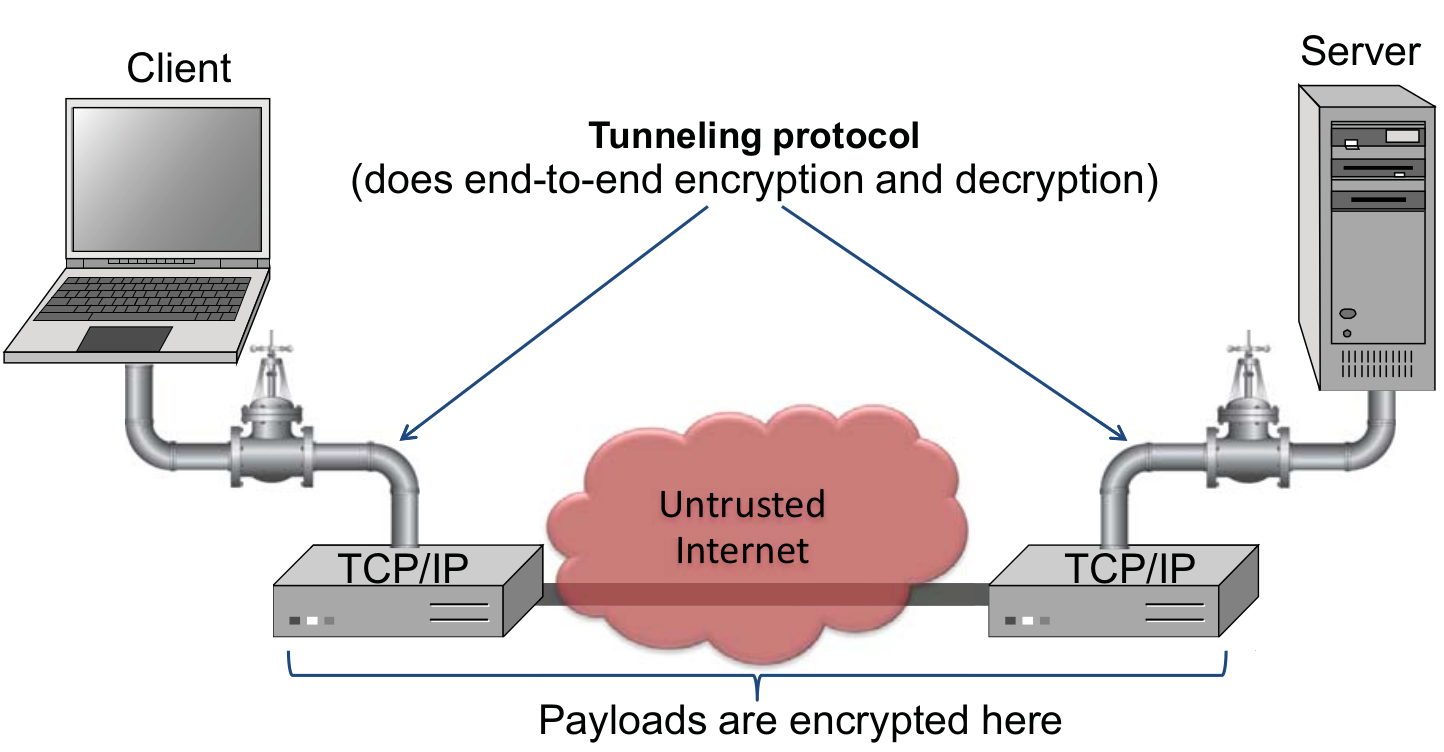
\includegraphics[height=13cm, width=13cm, keepaspectratio]{Immagini/firewalls/tunnel.png}}
	\caption{Stateful firewall \label{fig:tunnel}} 	
\end{figure}

\section{Intrusion Detection Systems (IDS)}
Un intrusion detection system (IDS) è un dispositivo o un'applicazione software che monitora le attività della rete o di un sistema identificando attività malevoli o violazione di policy, e produce dei report a riguardo.
Alcune definizioni:
\begin{itemize}
\item \textbf{Intrusione}: Azione finalizzata alla compromissione della sicurezza dell'obbiettivo (confidenzialità, integrità, disponibilità o risorse di rete e/o di calcolo)
\item \textbf{Intrusion detection}: L'identificazione, tramite segnali di intrusione e la relativa produzione di report a riguardo.
\item \textbf{Intrusion prevention}: Il processo che coinvolge sia la rivelazione di attività di intrusione sia la gestione automatica delle misure di reazione all'intrusione.
\end{itemize}

\subsection{Componenti di un IDS}
L'\textbf{IDS manager} processa i dati provenienti dai \textbf{sensori IDS} con il fine di determinare su è avvenuta un'intrusione. Tale rilevamento è basato su una serie di policy, ovvero di regole e condizioni che, se verificate, indicano una probabile intrusione. Una volta che il manager rileva un intrusione, scatta un allarme.

\begin{figure}[htbp]
	\centering
	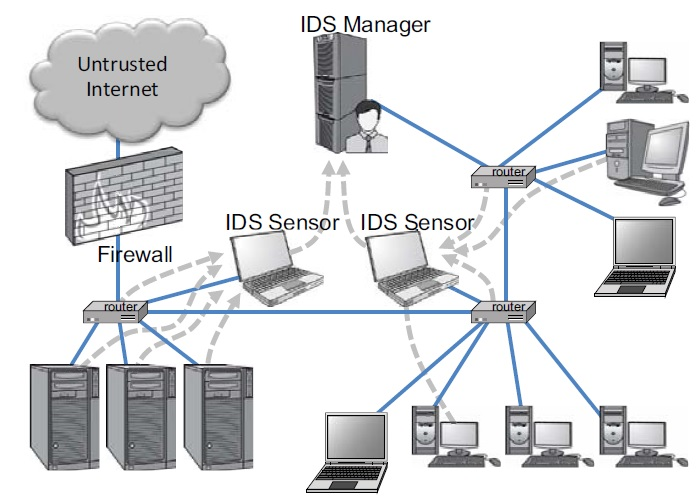
\includegraphics[width=0.5\linewidth]{Immagini/firewalls/IDS.png}
	\caption{IDS Components} 	
	\label{fig:IDS_components}
\end{figure}

\subsection{Intrusioni}
Un IDS è progettato al fine di rilevare una serie di minacce, tra cui le seguenti:

\begin{itemize}
\item \textbf{Masquerader}: un attaccante che sta utilizzando in maniera fraudolenta l'identità e/o le credenziali di un utente legittimo per ottenere accesso ad un computer o ad una rete
\item \textbf{Misfeasor}: un utente legittimo che sta eseguendo azione che non è autorizzato ad eseguire
\item \textbf{Clandestine user}: un utente che prova a bloccare o mascherare le sue azioni file di audit e/o log di sistema
\end{itemize}

Inoltre un IDS può essere progettato al fine di rilevare i seguenti attacchi automatizzati:
\begin{itemize}
\item \textbf{Port scans}: information gathering finalizzata a scoprire quali porte su una determinata interfaccia accettano connessioni TCP
\item \textbf{Denial-of-service attacks}: attacchi di rete finalizzati a saturare un host di richieste fino all'impossibilità di erogare il servizio che normalmente eroga
\item \textbf{Malware attacks}: Trojan horses, computer worms, virus, etc.
\item \textbf{ARP spoofing}: tentativi di reindirizzare traffico ip in una LAn
\item \textbf{DNS cache poisoning}: attacco che prevede la modifica della chache DNS di un host per creare una falsa associazione domain-name/IP-address 
\end{itemize}

\subsection{IDS Data} 
In una influente pubblicazione del 1987, Dorothy Denning identificò molti campi che dovrebbero essere inclusi nella registrazione degli eventi da parte di un IDS:
\begin{itemize}
\item \textbf{Subject}: l'iniziatore di un'azione sull'obbiettivo
\item \textbf{Object}: la risorsa in questione, come un file, un comando, un device, o un protocollo di rete
\item \textbf{Action}: l'operazione eseguita dal subject verso l'object
\item \textbf{Exception-condition}: ogni messaggio di errore o eccezione sollevata dalla action
\item \textbf{Resource-usage}: misure quantitative delle risorse utilizzate dal sistema nell'effettuare la action
\item \textbf{Time-stamp}: un identificatore unico per il momento nel tempo in cui si inizia la action
\end{itemize}

\subsection{Tipi di Intrusion Detection Systems} 
\subsubsection{Rule-Based Intrusion Detection} 
Rules identify the types of actions that match certain known profiles for an intrusion attack, in which case the rule would encode a signature for such an attack. Thus, if the IDS manager sees an event that matches the signature for such a rule, it would immediately sound an alarm, possibly even indicating the particular type of attack that is suspected.

\subsubsection{Statistical Intrusion Detection}
A profile is built, which is a statistical representation of the typical ways that a user acts or a host is used; hence, it can be used to determine when a user or host is acting in highly unusual, anomalous ways.
Once a user profile is in place, the IDS manager can determine thresholds for anomalous behaviors and then sound an alarm any time a user or host deviates significantly from the stored profile for that person or machine.

\section{Cross Site Scripting (XSS)}
Cross-site scripting is a type of computer security vulnerability typically found in Web applications. XSS enables attackers to \textbf{inject client-side script} into Web pages viewed by other users. It can be used for many types of attack: phishing, hijacking, changing of user settings, cookie theft/poisoning, false advertising, execution of code on the client, etc. 
\begin{figure}[htbp]
	\centering
	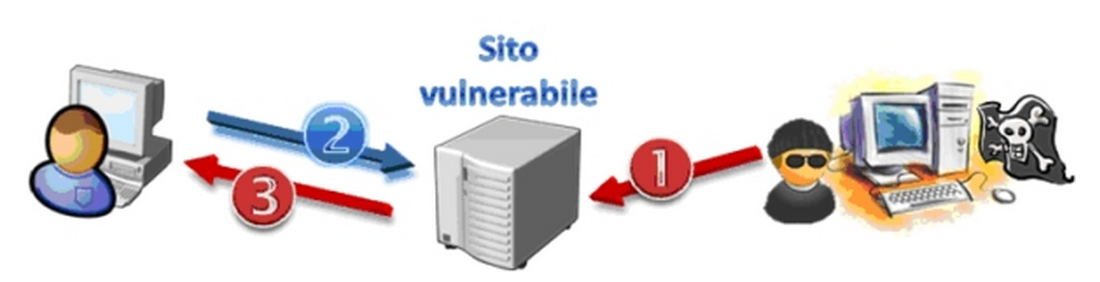
\includegraphics[width=0.5\linewidth]{Immagini/firewalls/XSS.png}
	\caption{Schema base di un attacco XSS} 	
	\label{fig:XSS_attack}
\end{figure}
\\
Methods for injecting malicious code are of three types:
\begin{itemize}
	\item \textbf{DOM-based (“type 0”)}: The attacker stores the malicious code locally in a standard object model for representing HTML or XML called the Document Object Model or DOM for short.
	\item \textbf{Reflected XSS (“type 1”)}: the attack script is reflected back to the user as part of a page from the victim site.
	\item \textbf{Stored XSS (“type 2”)}: the attacker stores the malicious code in a resource managed by the web application, such as a database.
\end{itemize}
Possible client-side XSS defenses are the following:
\begin{itemize}
	\item \textbf{Proxy-based}: analyze the HTTP traffic exchanged between user's web browser and the target web server by scanning for special HTML characters and encoding them before executing the page on the user's web browser (i.e. NoScript -	Firefox plugin).
	\item \textbf{Application-level firewall}: analyze browsed HTML pages for hyperlinks that might lead to leakage of sensitive information and stop bad requests using a set of connection rules.
	\item \textbf{Auditing system}: monitor execution of JavaScript code and compare the operations against high-level policies to detect malicious behavior.
\end{itemize}

\section{SQL Injection Attack}
Many web applications take user input from a form. Often this user input is used literally in the construction of a SQL query submitted to a database. For example:
\begin{lstlisting}
SELECT user 
FROM table
WHERE name = 'user input name'
\end{lstlisting}
A SQL injection attack involves placing SQL statements in the user input.
\subsubsection{Login Query: username and password} 
Here follows a standard query to check if the Login is correct:
\begin{lstlisting}
SELECT * 
FROM users 
WHERE user = '$usern' AND pwd = '$password'
\end{lstlisting}
If an attacker enter values for username/password as:
\begin{lstlisting}
$usern = "M' OR '1=1"
$password = "M' OR '1 = 1"
\end{lstlisting}
The resulting query will be:
\begin{lstlisting}
SELECT * 
FROM users 
WHERE user = 'M' OR '1=1' AND pwd = 'M' OR '1=1'
\end{lstlisting}
Result: you obtain the access!\\
Another query:
\begin{lstlisting}
SELECT user, pwd 
FROM users 
WHERE user = '$usern' 
\end{lstlisting}
If again:
\begin{lstlisting}
$usern = "M' OR '1=1" 
\end{lstlisting}
Result: you obtain the entire table!\\
To overcome this type of attack we have to check whether the result is one tuple only and the formal correctness of the result. \\
\linebreak
Considering another kind of malicious input, if there was:  
\begin{lstlisting} 
$usern="M' ; drop table user;"
\end{lstlisting}
Then we can use an \textbf{Escape method}, where all "malicious" characters will be changed.
Here it is shown an example: the following expression
\begin{lstlisting} 
Escape("t ' c") 
\end{lstlisting}
gives as a result:
\begin{lstlisting} 
"t \' c"
\end{lstlisting}
So, writing:
\begin{lstlisting} 
SELECT user, pwd 
FROM users 
WHERE user = '$usern'
\end{lstlisting}
and:
\begin{lstlisting} 
$usern = escape("M' ;drop table user;")
\end{lstlisting}
Gives, as result, the safe query:
\begin{lstlisting} 
SELECT user, pwd 
FROM users 
WHERE user='M\'drop table user;\''
\end{lstlisting}
\textbf{Solution} for SQL injection attack are: \textbf{Escape string} and \textbf{strict type verification}